% Created 2022-02-22 mar 16:09
% Intended LaTeX compiler: pdflatex
\documentclass[conference]{IEEEtran}
\usepackage[utf8]{inputenc}
\usepackage[T1]{fontenc}
\usepackage{graphicx}
\usepackage{longtable}
\usepackage{wrapfig}
\usepackage{rotating}
\usepackage[normalem]{ulem}
\usepackage{amsmath}
\usepackage{amssymb}
\usepackage{capt-of}
\usepackage{hyperref}
\input{~/org/latex/author_TeoCir2_Riedinger.tex}
\input{~/org/latex/ieee.tex}
\date{\today}
\title{Sistema de adquisión y transmisión de datos autosuficiente y controlable - Manual de Servicio}
\hypersetup{
 pdfauthor={},
 pdftitle={Sistema de adquisión y transmisión de datos autosuficiente y controlable - Manual de Servicio},
 pdfkeywords={},
 pdfsubject={},
 pdfcreator={Emacs 27.2 (Org mode 9.6)}, 
 pdflang={Spanish}}
\begin{document}

\maketitle
\tableofcontents


\section{Consideraciones de seguridad:}
\label{sec:orgdbc0214}
\subsection{Riesgos y procedimientos de seguridad:}
\label{sec:orgd3031b4}
Ambos sistemas operan niveles de bajos de voltaje, por lo que los riesgos al realizar los mantenimientos son mínimos. Sin embargo, se deben tener las siguientes precauciones al operar:

\begin{itemize}
\item Utilizar calzado y pulseras antiestáticas para evitar el daño a los equipos.
\item Desconectar de la alimentación ambos sistemas antes de realizar el mantenimiento (aunque sea de solo un sistema en particular).
\item Desconectar la conexión USART entre ambos sistemas antes de realizar el mantenimiento de uno de los mismos.
\end{itemize}
\section{Herramientas y equipos para realizar el servicio:}
\label{sec:org02bb197}
\subsection{Herramientas e instrumental necesario:}
\label{sec:orge3339a5}
Será necesario para realizar el mantenimiento las siguientes herramientas:

\begin{itemize}
\item Destornilladores tipo paleta y Philips para realizar el desamblaje de las carcasas de los equipos.
\item Multímetro digital o analógico para corroborar los valores de referencia (con el sistema encendido para realizar mediciones de voltaje y con el sistema desconectado para realizar mediciones de continuidad).
\item Osciloscopio digital u analógico para corroborar las señales de referencia (con el sistema conectado).
\item Manuales de usuario de los elementos anteriores y de los siguientes:
\begin{itemize}
\item STM32F429ZI-Nucleo.
\item LM35Z.
\item LM358.
\end{itemize}
\end{itemize}
\subsection{Software y aplicaciones necesarias:}
\label{sec:org8a55edb}
Para comprobar y debugger el código embebido en el sistema será necesario el programa libre de ST Atollic TRUEStudio. Indiferentemente, también es posible utilizar cualquiera de las opciones ofrecidas por ST o algún otro programa basado en Eclipse, pero se aclara que el programa de ambos sistemas fue debuggeado en Atollic TRUEStudio y solo probado en el mismo.

Luego, para editar los archivos del PCB será necesario el software Proteus 8.12 SP0 Professional.

Todos los archivos de software se pueden encontrar en la página oficial de GitHub del proyecto: \url{https://github.com/AugustoRiedinger/tecDig2\_project}.
\section{Diagramas de circuito}
\label{sec:org24ba558}
\subsection{Diagrama general en bloques:}
\label{sec:orgaff0334}
\begin{figure}[htbp]
\centering
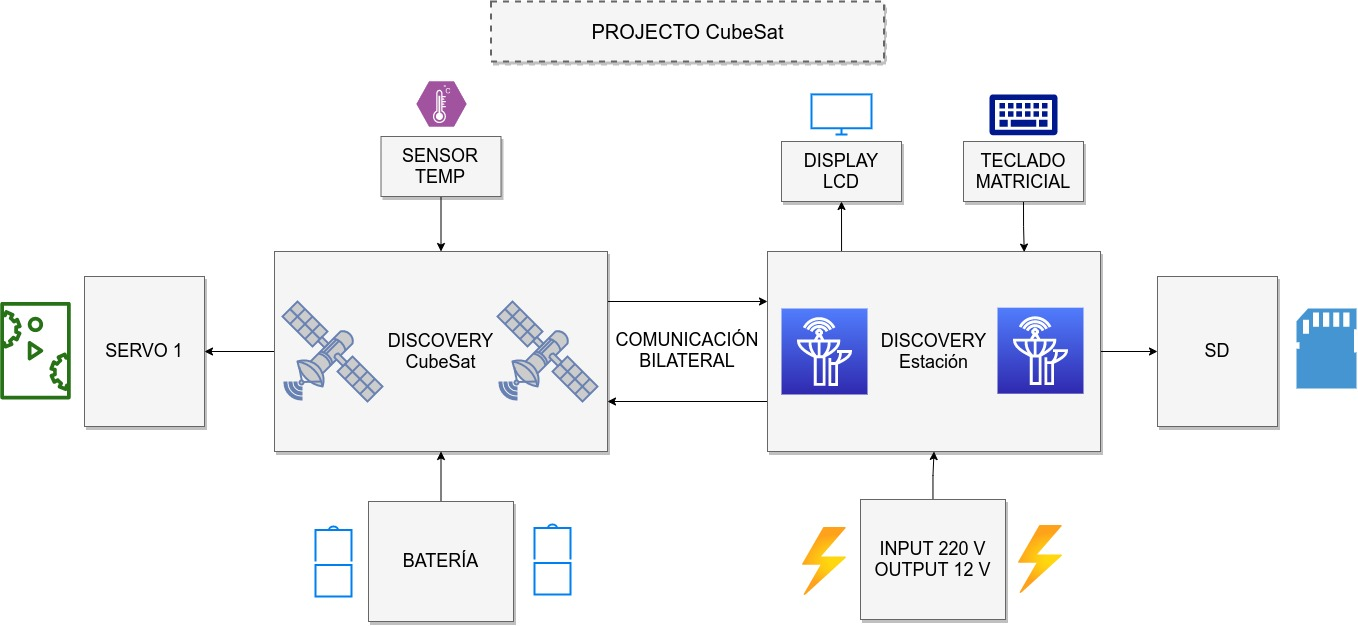
\includegraphics[width=.9\linewidth]{../../images/diagramaBloques.jpg}
\caption{\label{fig:diagramaBloques}Diagrama general en bloques}
\end{figure}
\end{document}
